% Chapter 3
\chapter{بلوغ محصولات}

پروتکل \lr{Openflow} در مسیر پیشرفت، با مشکلات بزرگی مواجه می‌شود. یکی از مشکلات این است که شرکت‌های تولید کننده نرم‌افزار و سخت‌افزار به دلیل وسعت دامنه تغییرات برای پشتیبانی، نمی‌توانند با سرعت پیشرفت پروتکل هماهنگ شوند. و مشکل دوم نیز از آنجایی نشئت می‌گیرد که پروتکل \lr{Openflow} تلاش دارد تا اکوسیستمی برای شبکه فراهم آورد که از تولید کننده سخت‌افزار مجزا است و در آن تجهیزات از شرکت‌های تولید کننده مختلف می‌توانند تحت یک کنترل کننده عمل کنند اما پس از عرضه پروتکل مشاهده می‌شود که حتی نسخه یکسانی از پروتکل که توسط چند شرکت متفاوت پیاده سازی شده‌اند نیز دارای تفاوت‌هایی در عملکرد و پیکربندی می‌باشد.\\
در زمان نگارش این گزارش، نسخه \lr{OF1.3} به صورت گسترده در تجهیزات و کنترل کننده‌های عملیاتی در حال استفاده است. نسخه \lr{OF1.4} در حال افزایش پشتیبانی و تعداد استفاده تجهیزات از آن است که در آینده نزدیک شاهد جایگزینی کامل \lr{OF1.3} با این نسخه خواهیم بود. اما با تغییرات عمده صورت گرفته در نسخه \lr{OF1.5} به ویژه تغییرات در خط لوله و اضافه شدن مرحله پردازشی خروجی، انتظار می‌رود روند همه‌گیر شدن استفاده از این نسخه به کندی صورت پذیرد. در حال حاضر سوئیچ‌های نرم‌افزاری مانند \lr{OvS} و برخی از برند‌های سخت افزار از این پروتکل پشتیبانی می‌کنند و تنها کنترل کننده که از این نسخه پشتیبانی می‌کند، \lr{Ryu SDN Controller} می‌باشد. در ادامه به معرفی دو محصول پشتیبانی کننده از نسخه \lr{OF1.5} یعنی سوئیچ \lr{OvS} و کنترل کننده \lr{ryu} می‌پردازیم.

\begin{figure}
	\centering
	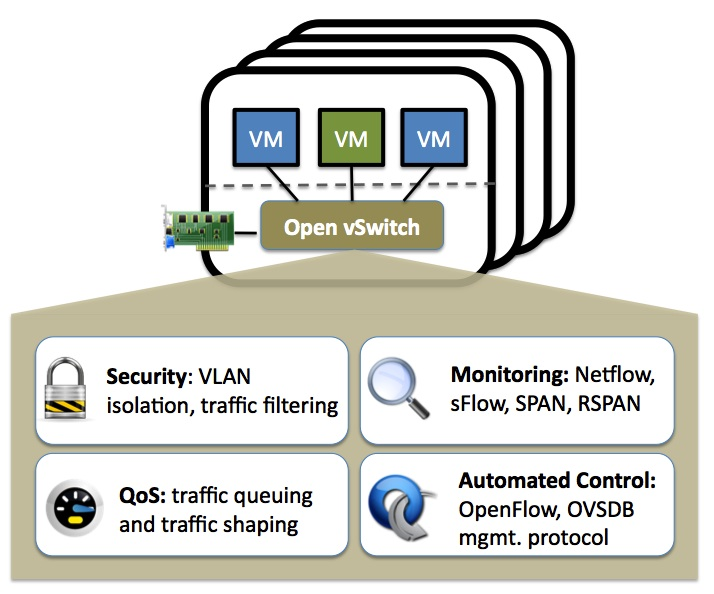
\includegraphics[scale=0.3]{imgs/ovs.jpg}
	\caption{نمایی از قابلیت‌های سوئیچ \lr{OvS} \cite{ovs}}
	\label{fig8}
\end{figure}


\section{\lr{Open vSwitch (OvS)}}
این سوئیچ در واقع پیاده سازی نرم افزاری منبع‌باز سوئیچ چندلایه شبکه است که توسعه‌ی آن توسط بنیاد آزاد لینوکس مدیریت می‌شود و تحت گواهی \lr{Apache 2.0} به صورت رایگان در دسترس می‌باشد. طراحی آن به گونه‌ای است که قابلیت ایجاد برنامه ریزی و خودکارسازی شبکه را در سطح گسترده و آماده برای بهره برداری فراهم می‌آورد. از قابلیت‌های مهم آن می‌توان به پیشتیبانی از سیستم‌عامل‌های مرسوم مانند لینوکس\LTRfootnote{Linux} و پلتفرم‌های مجازی سازی و شبکه مانند \lr{VMware} و \lr{Cisco} اشاره کرد.\\
آخرین نسخه پایدار منتشر شده از این سوئیچ، نسخه \lr{v2.14} می‌باشد که قابلیت پشتیبانی از \lr{OF1.5} را به صورت پیش فرض دارد.

\begin{figure}
	\centering
	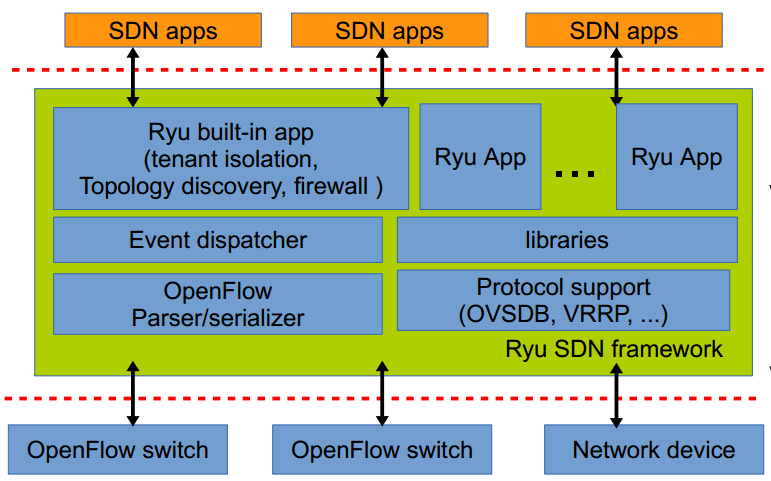
\includegraphics[scale=0.3]{imgs/ryu.png}
	\caption{نمایی از اجزاء تشکیل دهنده چهارچوب نرم افزاری \lr{Ryu}}
	\label{fig9}
\end{figure}

\section{\lr{RYU sdn controller}}
ری-هو (\lr{Ryu})، یک چهارچوب مولفه محور به منظور توسعه شبکه‌های مبتنی بر نرم افزار می‌باشد که قادر به تولید نرم افزار‌هایی برای کنترل و مدیریت شبکه‌ها است. این کنترل کننده از پروتکل‌هایی مانند \lr{Openflow}، \lr{Netconf}، \lr{OF-conf} و غیره پشتیبانی می‌نماید. این نرم افزار به صورت آزاد و منبع باز تحت گواهی \lr{Apache 2.0} قابل دسترسی است.\\
توسعه در این چهارچوب توسط رابط نرم‌افزاری\LTRfootnote{API} با زبان پایتون\LTRfootnote{Python} انجام می‌پذیرد. شکل \ref{fig9} نشان دهنده اجزاء تشکیل دهنده این چهارچوب و محل قرارگیری برنامه‌های توسعه یافته توسط کاربر را نشان می‌دهد \cite{ryu_site}.

\section{آزمایش پشتیبانی سوئیچ از نسخه \lr{OF1.5}}
در این قسمت به بررسی پشتیبانی سوئیچ \lr{OvS} نسخه \lr{v2.14.2} از پروتکل \lr{Openflow} نسخه \lr{OF1.5} توسط کنترل کننده \lr{Ryu} نسخه \lr{v4.34} می‌پردازیم. در حال حاظر تنها تجهیزات و کنترل کننده‌های پشتیبانی کننده از نسخه نهایی \lr{OF1.5}، نرم افزار‌های فوق الذکر می‌باشند که حتی پلتفرم‌های آزمایش پیروی از نسخه پروتکل\LTRfootnote{Protocol Conformance Test} نیز برای آن موجود نمی‌باشد. در ادامه این آزمایش به نمایش کارکرد نرم افزار‌‌های فوق می‌پردازیم.

\begin{figure}[H]
	\centering
	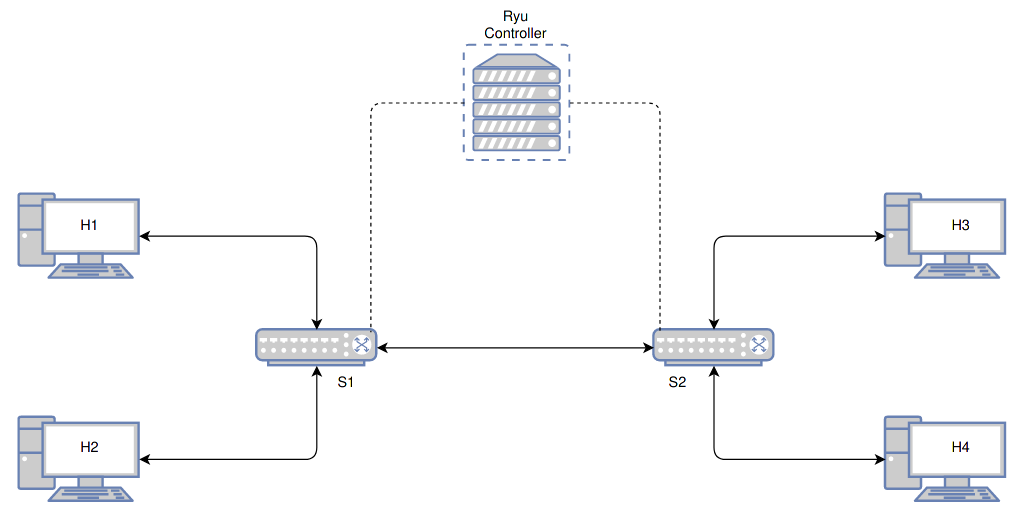
\includegraphics[scale=0.4]{imgs/of15_test.png}
	\caption{نمایی از سناریو شبیه سازی شده}
	\label{fig10}
\end{figure}

\subsection{محیط شبیه سازی}
کنترل کننده \lr{Ryu} در یک محیط کانتینری به نام \lr{Docker} با آدرس آيپی\LTRfootnote{IP} \lr{\texttt{172.17.0.2}} و یک برنامه کاربردی به منظور ایجاد عملکرد یک سوئیچ لایه ۲ شبکه درون آن در حال اجرا می‌باشد. سوئیچ‌های \lr{OvS} نیز توسط برنامه شبیه ساز \lr{Mininet} ایجاد شده‌اند و با  کنترل کننده توسط آدرس آیپی \lr{\texttt{172.17.0.1}} در ارتباط هستند و سناریو شکل \ref{fig10} نشان دهنده بخش‌های موجود در شبیه سازی می‌باشد.\\
حال با استفاده از نرم افزار شنود شبکه به نام \lr{Wireshark}، بسته‌های رد و بدل شده بین کنترل کننده و سوئیچ را بررسی می‌کنیم.

\begin{figure}
	\centering
	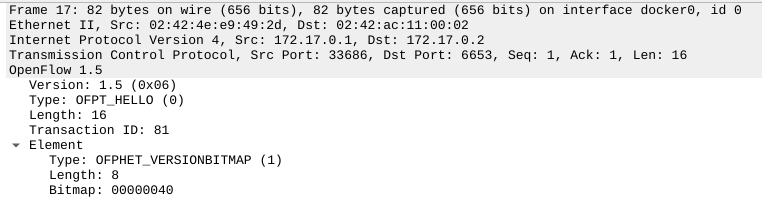
\includegraphics[scale=0.5]{imgs/s_c_hello.png}
	\caption{پیام ارسالی \lr{HELLO} از سوئیچ به کنترل کننده}
	\label{fig11}
\end{figure}

\begin{figure}
	\centering
	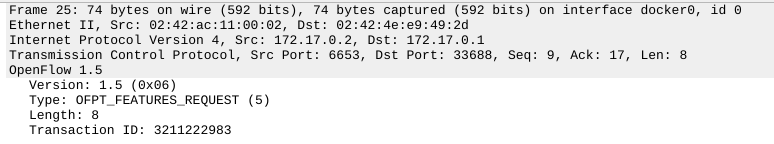
\includegraphics[scale=0.5]{imgs/c_s_fr.png}
	\caption{پیام ارسالی \lr{FEATURES\_REQUEST} از کنترل کننده به سوئیچ}
	\label{fig12}
\end{figure}

همانطور که در شکل \ref{fig11} مشاهده می‌کنیم یک نمونه از پیام ارسالی از سوئیچ به کنترل کننده می‌باشد که نسخه پروتکل را \lr{OF1.5} نشان می‌دهد و همچنین شکل \ref{fig12} نیز یک نمونه از پیام ارسالی از کنترل کننده به سوئیچ است و نسخه این پیام نیز \lr{OF1.5} می‌باشد که نشان دهنده پشتیبانی این دو نرم افزار از نسخه جدید می‌باشد.

\subsection{ایجاد عملکرد شبه دیوار آتش}
با استفاده از قابلیت جدید \lr{TCP\_Flags Match} در نسخه \lr{OF1.5} می‌توان سیاست‌های مرتبط با اتصالات \lr{TCP} اعمال کرد. برای نمایش این قابلیت ابتدا به توضیح یک نوع پویش شبکه\LTRfootnote{Network Scan} به نام \lr{Xmas Scan} می‌پردازیم. طبق این پویش به منظور یافتن دستگاه‌ها و سرویس‌های موجود در شبکه، پرچم‌های \lr{FIN,PSH,URG} در بسته فعال می‌گردند. برای جلوگیری از انجام این پویش در شبکه، می‌توان در سناریو بخش قبل از \lr{TCP\_Flags Match} به منظور یافتن بسته‌های مربوط به این پویش و حذف آن‌ها اقدام کرد.\\
به این منظور، توسط کنترل کننده یک مدخل جریان در جدول جریان سوئیچ‌ها به شرح زیر ایجاد می‌کنیم:
\begin{flushleft}
	\lr{\texttt{priority=20,tcp,tcp\_flags=fin|psh|urg actions=drop}}
\end{flushleft}
با اجراء دستور زیر، نتیجه را قبل و بعد از ایجاد مدخل جریان فوق در شکل‌های \ref{fig13} و \ref{fig14} مشاهده می‌کنیم:
\begin{flushleft}
	\lr{\texttt{nping --count 1 --tcp --flags fin,psh,urg  10.0.0.2}}
\end{flushleft}

\begin{figure}
	\centering
	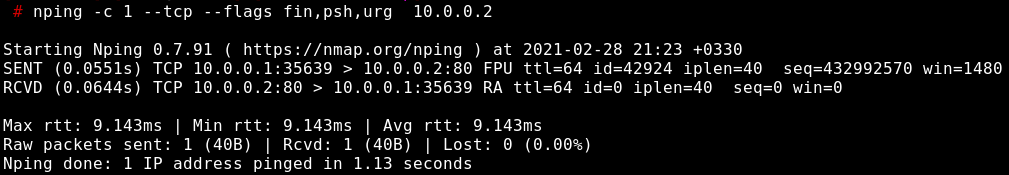
\includegraphics[scale=0.5]{imgs/tcp_b.png}
	\caption{ارسال درخواست قبل از ایجاد مدخل جریان}
	\label{fig13}
\end{figure}
\begin{figure}
	\centering
	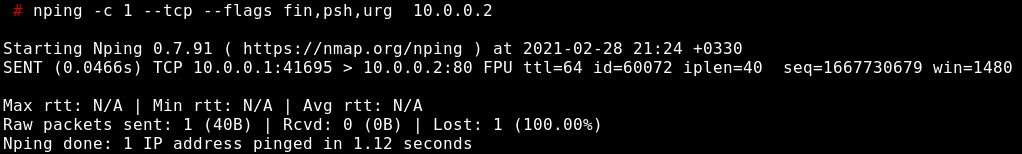
\includegraphics[scale=0.5]{imgs/tcp_a.png}
	\caption{ارسال درخواست بعد از ایجاد مدخل جریان}
	\label{fig14}
\end{figure}

همانطور که طی آزمایش مشاهده شد، بسته‌ها به سمت آدرس مورد نظر ارسال نشدند اما باقی بسته‌هایی که پرچم‌های مربوطه را ندارد بدون مشکل ارسال و دریافت می‌شوند.







